\section*{Sistemas con \(N\gg 1\) grados de libertad forzados}

				
\item
\begin{minipage}[t][3.5cm]{0.6\textwidth}
Este arreglo lineal de péndulos acoplados tiene extremos en $z= 0$ y en $z= L$.
Se aplica una fuerza externa en función del tiempo a la primera masa ($z=0$), de forma tal que se conoce su amplitud $\psi(0,t)= A_0 \cos(\Omega t)$.
Halle el movimiento estacionario del sistema y discuta las hipótesis que hace.
Compare con el caso de extremo derecho fijo a una pared (o sea: agregando un resorte a la derecha de la última masa y uniéndolo a la pared). 
\end{minipage}
\begin{minipage}[c][0cm][t]{0.35\textwidth}
  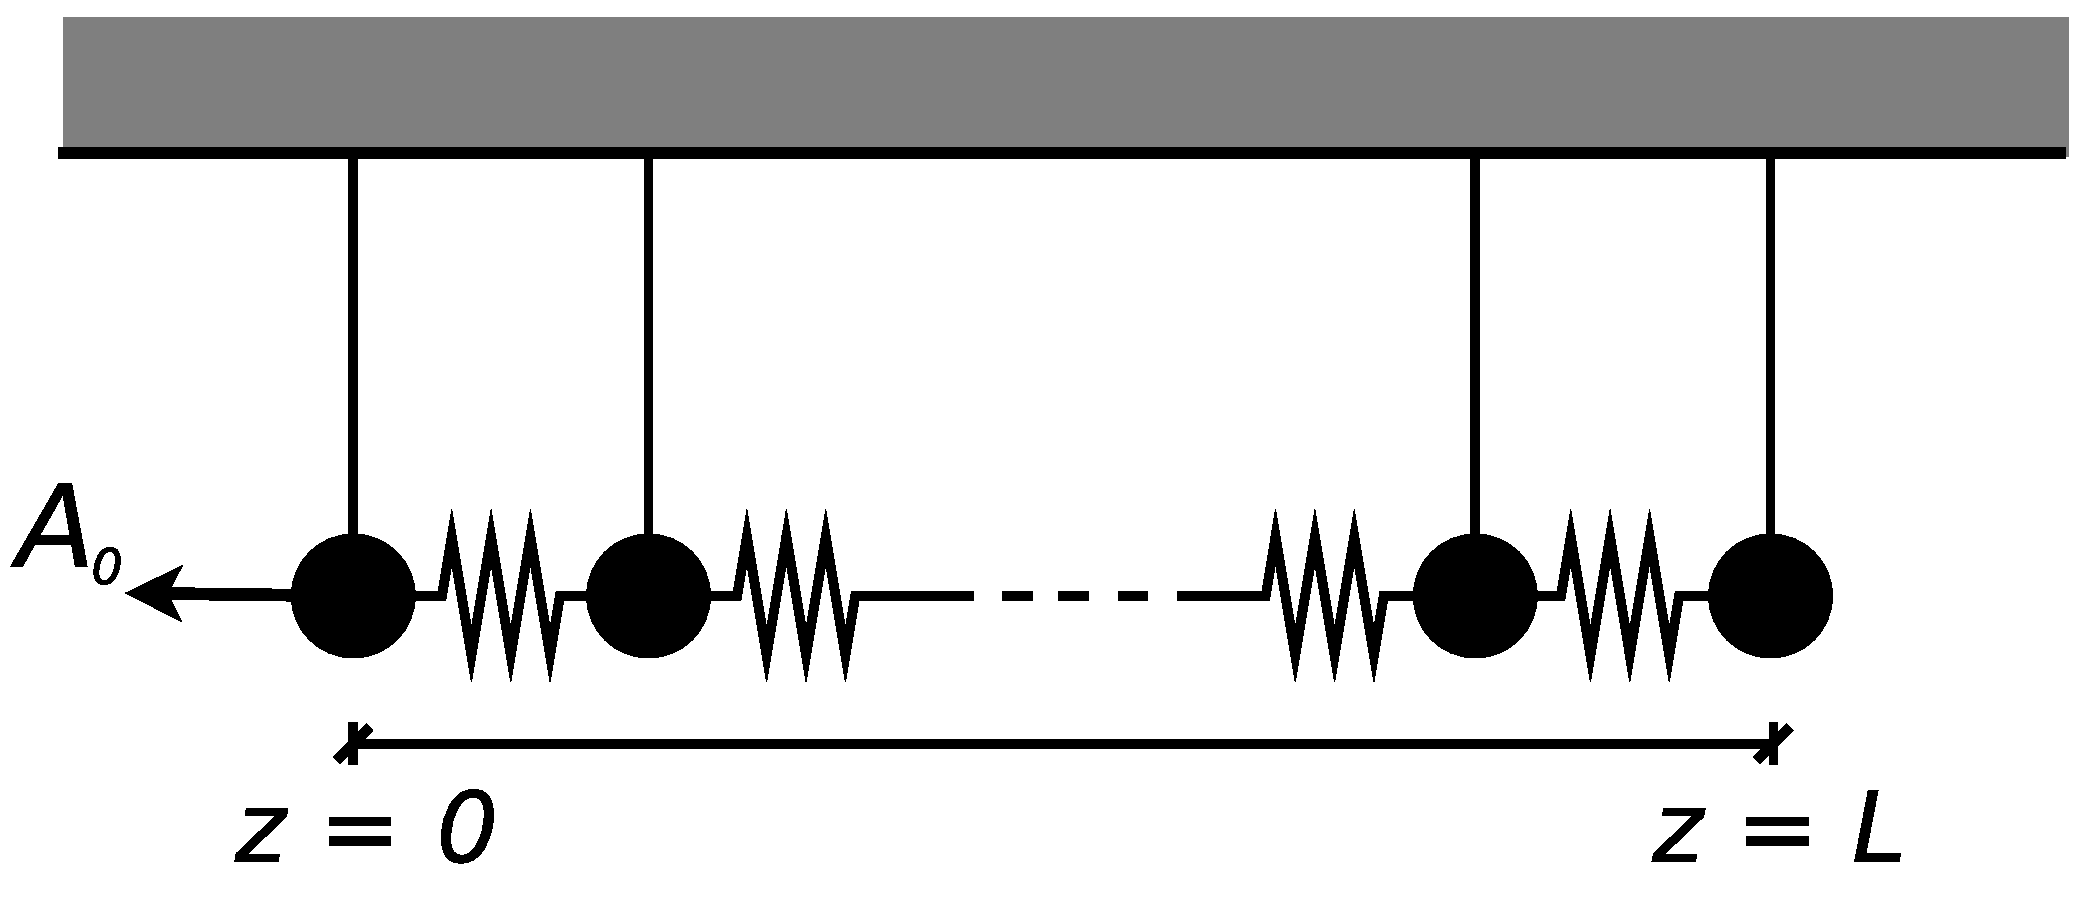
\includegraphics[width=\textwidth]{ej1-15}
\end{minipage}



\item
\begin{minipage}[t][3cm]{0.35\textwidth}
Considere un sistema de péndulos acoplados con un cambio brusco en $\omega_{0}^{2}$ en $z=L$, según se esquematiza en la figura.
\end{minipage}
\begin{minipage}[c][3cm][t]{0.6\textwidth}
  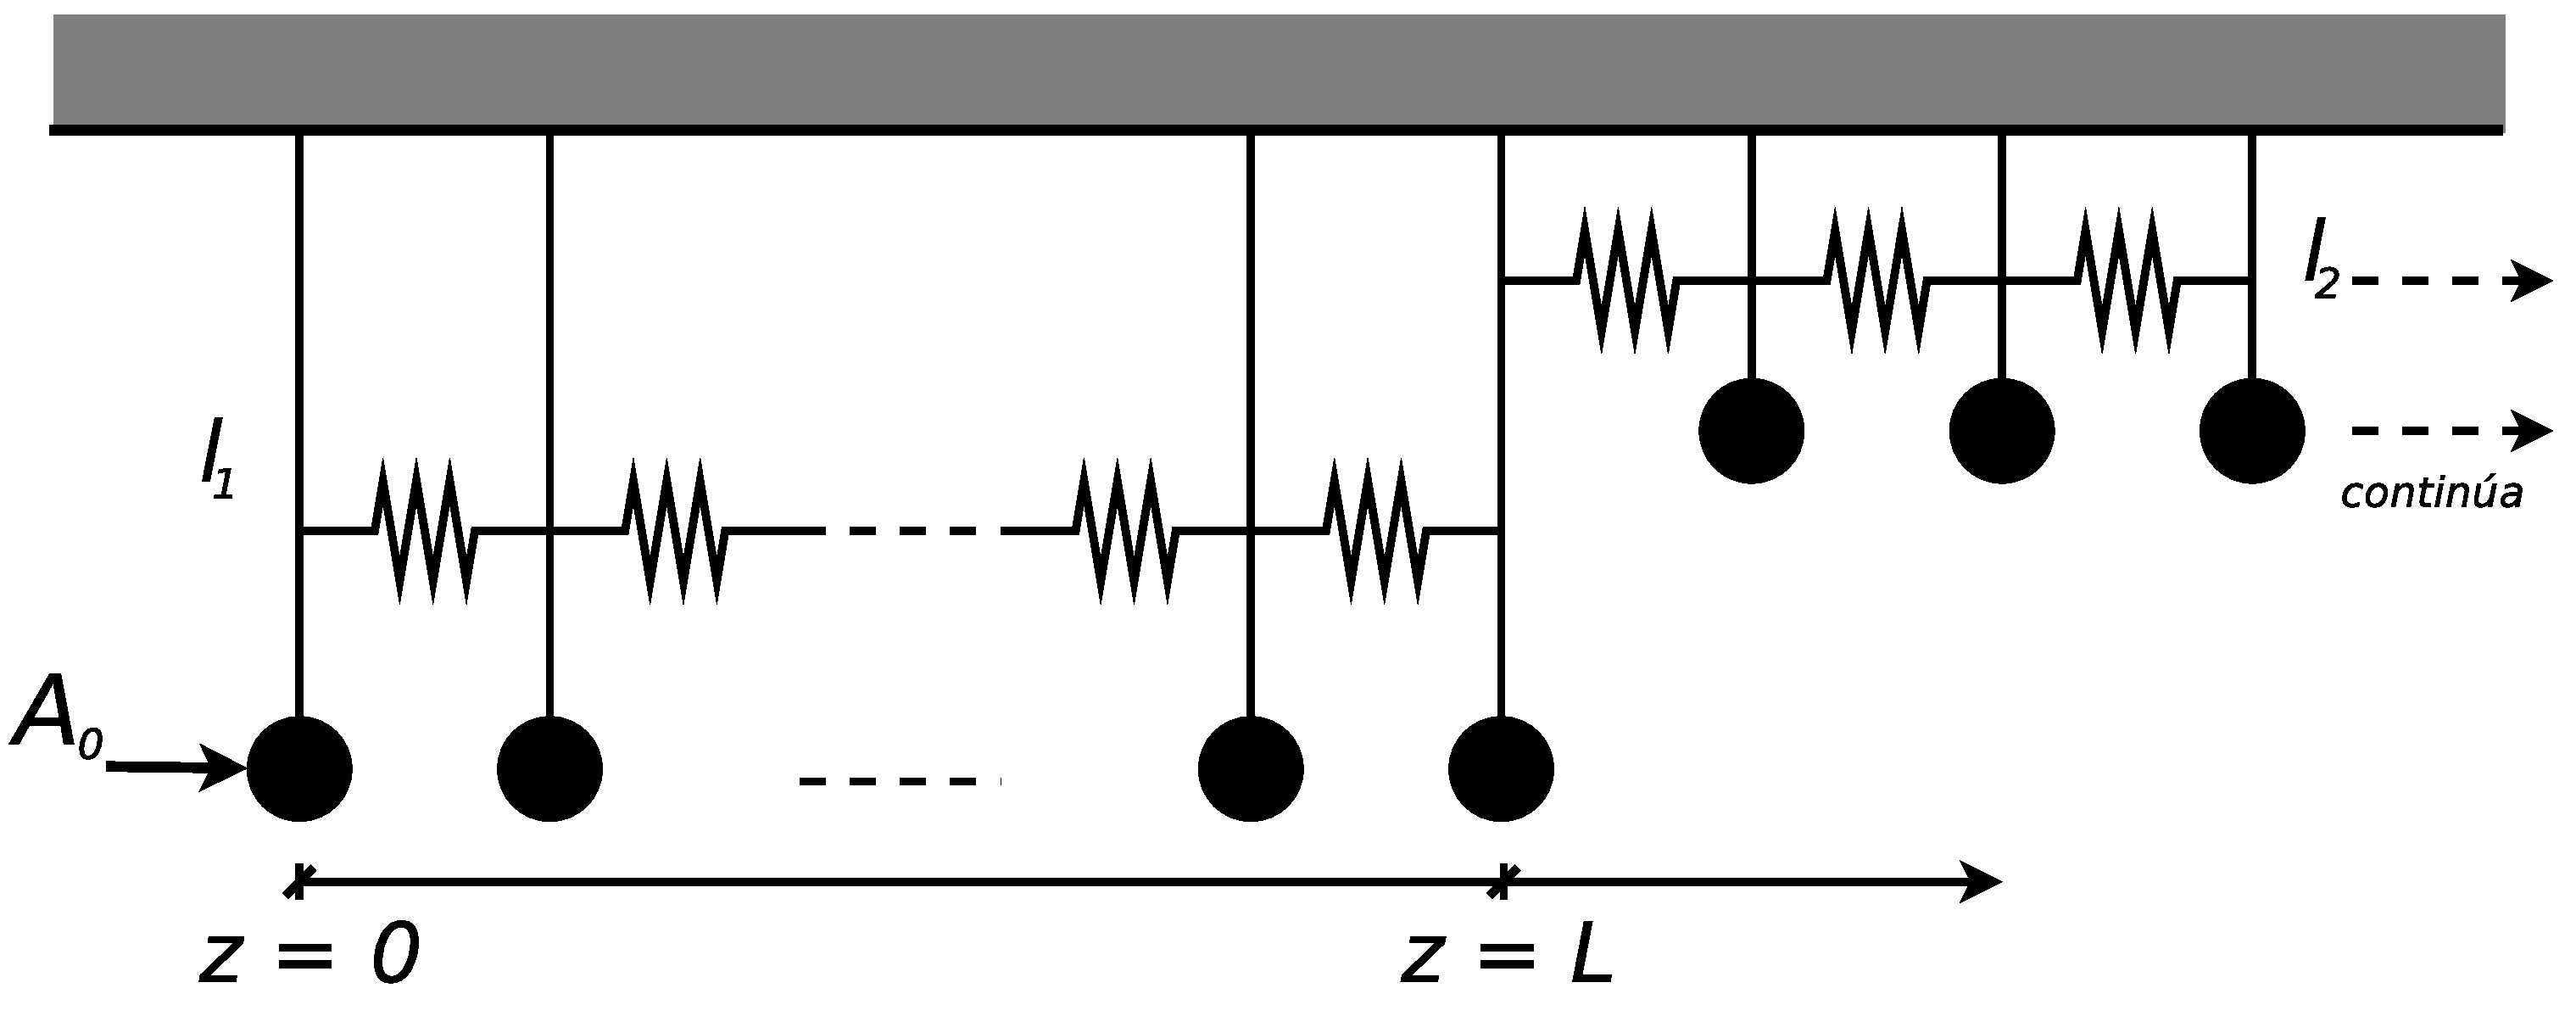
\includegraphics[width=\textwidth]{ej1-16}
\end{minipage}
\begin{enumerate}
	\item Discuta cómo tiene que ser \(\Omega\) para que el sistema se comporte como dispersivo en \(0< z < L\) y reactivo en \(z > L\).
	¿Cuál sería la relación entre \(l_1\) y\(l_2\)?
	\item En dichas condiciones estudie el movimiento estacionario del sistema y encuentre las frecuenciasde resonancia.
	\item ¿Qué pasa ahora si se invierte la relación entre \(l_1\) y \(l_2\)?
	¿De qué variable depende el comportamiento en \(z > L\)?
	\item ¿Es posible encontrar un rango de frecuencias \(\Omega\) tal que el sistema se encuentre en el mismo rango de comportamiento en \(0< z < L\) y en \(z > L\)?
\end{enumerate}



\item
\begin{minipage}[t][3.5cm]{0.45\textwidth}
Para el sistema esquematizado en la figura, calcule $\psi_{n}(t)$, si $\Omega<\omega_\textrm{mín}$, es decir que se fuerza con una frecuencia menor que la propia del sistema en su modo fundamental de oscilación.
\end{minipage}
\begin{minipage}[c][2cm][t]{0.5\textwidth}
  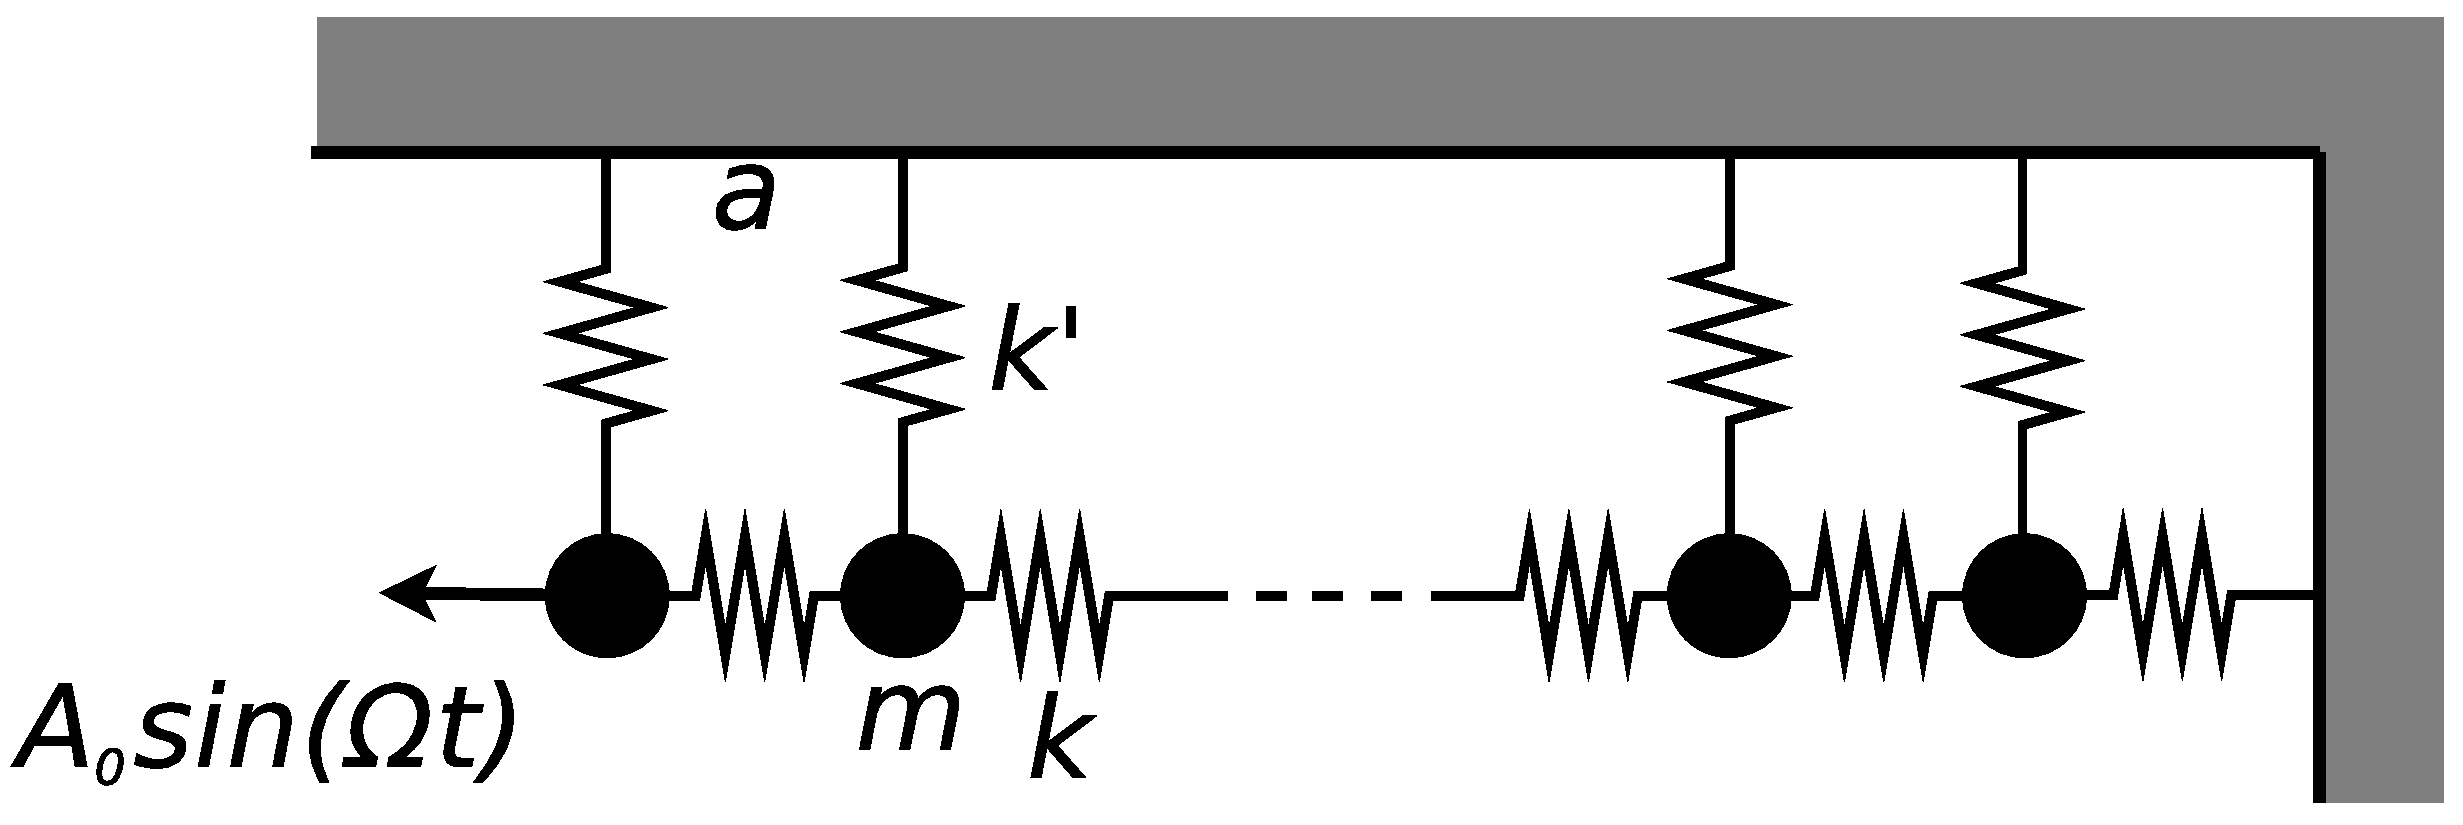
\includegraphics[width=\textwidth]{ej1-17}
\end{minipage}
